\section{LTI系统的微分方程模型}

很多物理系统,如电路、钟摆、悬挂等,其变量间存在导数和积分关系,整个系统可用微分方程描述,所以微分方程模型关键在于建模和求解微分方程。

本节要点:
\begin{itemize}
    \item 掌握微分方程的概念;
    \item 掌握一阶常系数线性微分方程的求解思路。
\end{itemize}

%============================================================
\subsection{微分方程的概述}

若LTI系统是有限维度,则可以用线性常系数微分方程描述如下:
\[
y^{\left( n \right)}\left( t \right) +\sum_{i=0}^{n-1}{A_iy^{\left( i \right)}\left( t \right)}=\sum_{i=0}^m{B_ix^{\left( i \right)}\left( t \right)}
\]
其中,$A_i,B_i$是实数,$n$称为{\bf 系统的阶}(order)。
配合初始条件,即可求出输入输出的对应关系。
特别地,我们称
\[
y\left( t \right) =B_0x\left( t \right)
\]
这样的系统为{\bf 静态系统},即输出只与当刻的输入有关。
静态系统过于简单,不予讨论。
如果系统的输出不仅与当刻输入有关,更与前刻输入有关,则称为{\bf 动态系统},动态系统的时域模型必为微分方程。
通常简单的微分方程可以求解,复杂的方程非常难解,特别是高阶的,甚至没有解析解。

一般来讲,真实系统多多少少都会将输入信号的能量在系统内部有暂留,相当于输出的能量在系统内部“来回振荡”了几下叠合起来再输出,所以在时域模型上,都会体现成微分方程,至少是一阶。

%============================================================
\subsection{一阶常系数线性方程的求解}

\begin{tcolorbox}
为了方便求解,时域分析(本章和下一章的卷积)的大量例子都是以一阶微分方程为例,所以这里特别讨论一阶常系数线性方程的求解方法。
微积分中的一阶常系数线性微分方程是关于一元函数$y=y\left( x \right) $的方程。
信号与系统中不一样,同样是一元函数,但是是$t$的参数方程$x=x\left( t \right) ,y=y\left( t \right) $。
\end{tcolorbox}

考虑如下形式的微分方程(一阶、常系数、非齐次):
\[
\frac{dy}{dt}+Py=Qx \qquad t\geqslant t_0
\]
\begin{itemize}
    \item $x=x\left( t \right) ,y=y\left( t \right) $:时间$t$的函数,表示输入信号和输出信号;
    \item $P,Q$:常实数。
\end{itemize}

采用变量替换法求解,首先两边同乘系数$e^{Pt}$:
\begin{align*}
&\because e^{Pt}\left( \frac{dy}{dt}+Py \right) =e^{Pt}Qx \\
&\therefore \frac{d}{dt}\left( e^{Pt}y \right) =Q\left( e^{Pt}x \right)
\end{align*}
变量替换$Y=e^{Pt}y,X=e^{Pt}x$,解得:
\begin{align*}
&\frac{d}{dt}Y=QX \\
&Y=Y\left( t_0 \right) +Q\int_{t_0}^t{Xd\tau}
\end{align*}
替换回,最终得到一阶微分方程的通解:
\begin{align*}
y\left( t \right) &=e^{-P\left( t-t_0 \right)}y\left( t_0 \right) +Qe^{-Pt}\int_{t_0}^t{e^{P\tau}x\left( \tau \right) d\tau} \qquad t\geqslant 0 \\
&=e^{-Pt}\left[ e^{Pt_0}y\left( t_0 \right) +Q\int_{t_0}^t{e^{P\tau}x\left( \tau \right) d\tau} \right]
\end{align*}
输出由两部分组成:
\begin{itemize}
    \item $e^{-Pt}e^{Pt_0}y\left( t_0 \right) $:对初始条件的响应,呈指数形式衰减;
    \item $e^{-Pt}Q\int_{t_0}^t{e^{P\tau}x\left( \tau \right) d\tau}$:对输入的响应,具体需要看输入的形式,但同样也是呈指数形式衰减。
\end{itemize}

%============================================================
\subsection{例RC电路}

\begin{example}
如下电路,假设系统零状态,若输入为单位阶跃信号$x=u\left( t \right) $,求系统的输出。
\end{example}

\begin{figure}[h]
\centering
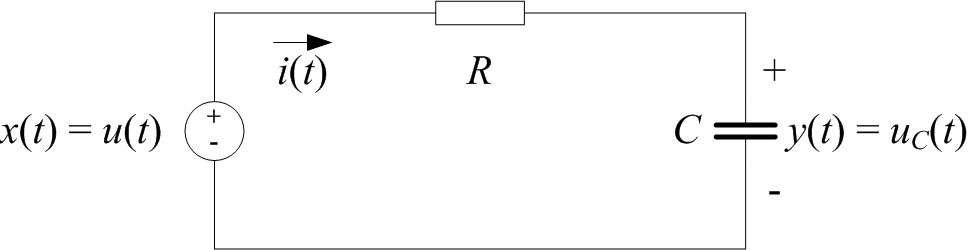
\includegraphics[height=2cm]{1.5.1-1.png}
\end{figure}

根据之前的分析,系统的微分方程模型:
\[
\frac{dy}{dt}+\frac{1}{RC}y=\frac{1}{RC}x \qquad \begin{cases}
	x\left( t \right) =u\left( t \right)\\
	y\left( 0^- \right) =0\\
\end{cases}
\]
求解该微分方程得到输出信号:
\begin{align*}
y\left( t \right) &=e^{-Pt}\left[ e^{Pt_0}y\left( t_0 \right) +Q\int_{t_0}^t{e^{P\tau}x\left( \tau \right) d\tau} \right] \\
&=e^{-\frac{1}{RC}t}\left[ y\left( 0 \right) +\frac{1}{RC}\int_0^t{e^{\frac{1}{RC}\tau}u\left( \tau \right) d\tau} \right] \\
&=\frac{1}{RC}e^{-\frac{1}{RC}t}\left[ \int_0^t{e^{\frac{1}{RC}\tau}d\tau} \right] =\frac{1}{RC}e^{-\frac{1}{RC}t}\left[ \left. RCe^{\frac{1}{RC}\tau} \right|_{0}^{t} \right] \\
&=1-e^{-\frac{t}{RC}} \qquad t\geqslant 0
\end{align*}
画图如下,可见,减小电阻或电容都可以提高输出对输入的“跟随性”。

\begin{python}
t  = np.arange(0, 10, 0.01)
RC = 1;   y1 = 1 - np.exp(-1 * t / RC)
RC = 0.1; y2 = 1 - np.exp(-1 * t / RC)

ax.plot(t, y1,       label='RC=1')
ax.plot(t, y2, '--', label='RC=0.1')
\end{python}

\begin{figure}[h]
\centering
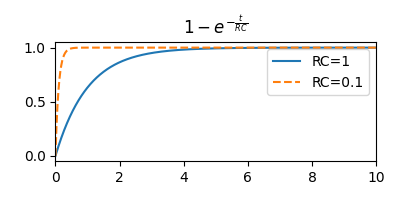
\includegraphics[height=3cm]{2.1.3-1.png}
\end{figure}




